\documentclass[12pt]{article}

% ---------------------------------------------------------------------------
% FAITH-SAE -- From First Principles: A Plain-Language Primer
% Vision interpretability: sparse autoencoders, causal faithfulness, OOD shift.
% Single column, generous margins, warm and inviting (NOT IEEE two-column).
% ---------------------------------------------------------------------------

\usepackage[utf8]{inputenc}
\usepackage[T1]{fontenc}
\usepackage{lmodern}
\usepackage[a4paper,margin=1.15in]{geometry}
\usepackage{amsmath,amssymb}
\usepackage{graphicx}
\usepackage{xcolor}
\usepackage{enumitem}
\usepackage{microtype}
\usepackage[most]{tcolorbox}
\usepackage[colorlinks=true,linkcolor=accent,urlcolor=accent,citecolor=accent]{hyperref}

% ---- palette ----
\definecolor{accent}{RGB}{38,90,160}
\definecolor{onman}{RGB}{38,120,90}       % on-manifold / good = green
\definecolor{offman}{RGB}{198,93,40}      % off-manifold / artifact = orange
\definecolor{boxbg}{RGB}{244,247,251}
\definecolor{boxrule}{RGB}{38,90,160}
\definecolor{ahabg}{RGB}{255,249,238}
\definecolor{aharule}{RGB}{198,93,40}
\definecolor{graytext}{RGB}{110,110,110}

% ---- line spacing, paragraph style ----
\renewcommand{\baselinestretch}{1.08}
\setlength{\parskip}{0.55em}
\setlength{\parindent}{0pt}

% ---- highlight boxes ----
\newtcolorbox{keybox}[1][]{
  colback=boxbg, colframe=boxrule, boxrule=0.6pt, arc=2.5pt,
  left=10pt, right=10pt, top=8pt, bottom=8pt, #1}
\newtcolorbox{ahabox}[1][]{
  colback=ahabg, colframe=aharule, boxrule=0.9pt, arc=2.5pt,
  left=10pt, right=10pt, top=8pt, bottom=8pt, #1}

% ---- a compact "definition / analogy / example" macro set ----
\newcommand{\dlabel}[1]{\textbf{\textcolor{accent}{#1}}\;}
\newcommand{\onm}[1]{\textcolor{onman}{#1}}
\newcommand{\offm}[1]{\textcolor{offman}{#1}}

% ---- section look ----
\usepackage{titlesec}
\titleformat{\section}{\Large\bfseries\color{accent}}{\thesection.}{0.5em}{}
\titleformat{\subsection}{\large\bfseries}{\thesubsection}{0.5em}{}
\titlespacing{\section}{0pt}{1.4em}{0.5em}

% ---- footer ----
\usepackage{fancyhdr}
\pagestyle{fancy}
\fancyhf{}
\fancyfoot[C]{\small\textcolor{graytext}{For research and educational purposes only.}}
\fancyfoot[R]{\small\textcolor{graytext}{\thepage}}
\renewcommand{\headrulewidth}{0pt}
\renewcommand{\footrulewidth}{0.4pt}

% ===========================================================================
\begin{document}

% ----------------------------- TITLE ---------------------------------------
\begin{center}
{\LARGE\bfseries\color{accent} FAITH-SAE: Are a Vision Model's ``Concept Switches'' Telling the Truth?}\\[0.35em]
{\large\itshape From First Principles: A Plain-Language Primer}\\[0.9em]
{\large Rajia Rani}\\[0.2em]
{\small\textcolor{graytext}{}}\\[0.3em]
{\small\textcolor{graytext}{A teaching primer --- built from zero, no specialist knowledge assumed.}}
\end{center}

\vspace{0.4em}
\hrule
\vspace{1.0em}

% ============================ SECTION 1 ====================================
\section{What you'll be able to explain after reading this}

This primer builds one modern research idea from the ground up. By the end, you should be able to walk to a whiteboard and explain, in your own words:

\begin{itemize}[leftmargin=1.4em, itemsep=2pt]
  \item \textbf{What a ``concept switch'' inside a vision AI is} --- how a tool called a \emph{sparse autoencoder} pulls thousands of hidden, human-readable concepts (``stripes,'' ``wheel,'' ``is-a-dog'') out of a frozen image model.
  \item \textbf{Why flipping such a switch can lie to you} --- the difference between an edit that produces a \emph{real} causal effect and one that produces a convincing \emph{fake} because it pushed the model somewhere no real image ever goes (``off-manifold'').
  \item \textbf{How to score honesty with one number} --- the \emph{Causal Faithfulness Score} (CFS), which asks three questions at once: does the effect grow smoothly, stay on-target, and reach the size it claims?
  \item \textbf{Why honesty can collapse on weird inputs} --- what ``out of distribution'' (sketches, corrupted photos, new domains) means, and why a switch that is faithful on clean photos may quietly stop telling the truth there.
\end{itemize}

You do \emph{not} need any machine-learning background. If you remember that a computer stores lists of numbers and that an arrow can point in a direction, you have enough.

% ============================ SECTION 2 ====================================
\section{The idea in 30 seconds}

Modern image AIs are black boxes: they work, but we can't see \emph{why}. A clever tool called a \emph{sparse autoencoder} cracks one open and finds thousands of internal ``switches,'' each seeming to stand for a human concept --- one for ``stripes,'' one for ``wheel,'' one for ``furry.'' Exciting! But there's a trap. If you flip a switch up and the picture's score for ``dog'' goes up, did you \emph{really} find the dog-concept --- or did you just shove the model into nonsense-land where its numbers misbehave and only \emph{look} like a dog effect?

This project does two things. \textbf{(A)} It flips switches \emph{carefully}, keeping the edit inside the space of settings that real images actually produce (``on-manifold'' steering), so the effect is real instead of a glitch. \textbf{(B)} It grades the result with a single honesty score, the \textbf{Causal Faithfulness Score}, and then asks the crucial follow-up: \emph{does that honesty survive when the test images get weird} --- sketches, blur, snow, unfamiliar scenes? The answer (a curve of honesty-versus-weirdness) tells us whether we can trust these concept switches in the real world, or only in the lab.

The rest of this document earns every phrase in that paragraph from first principles.

% ============================ SECTION 3 ====================================
\section{Foundations from zero}

Before the clever part, we need five plain ideas: what a \emph{frozen vision model} is, what its \emph{activations} are, what a \emph{sparse autoencoder} does, what it means to \emph{steer} a concept, and what ``on the manifold'' even means. Each comes as a \emph{definition}, an \emph{analogy}, and a \emph{tiny example}.

\subsection{What a frozen vision model is}

\dlabel{Definition.} A \emph{vision model} is a program that has already learned, from millions of labelled photos, to turn an image into useful internal numbers (and often a guess like ``this is a Labrador''). \emph{Frozen} means we have stopped training it: its knowledge is fixed, we never change a single one of its internal weights. We only \emph{observe} and \emph{poke} it. Throughout, picture a specific one --- CLIP ViT-B/16, a popular off-the-shelf image model.

\dlabel{Analogy.} A frozen model is like a fully-trained, retired expert chef who will no longer learn new recipes. We can watch what they do and occasionally nudge their hand mid-stir, but we never re-educate them.

\dlabel{Tiny example.} Show the frozen model a photo of a zebra. It will not learn anything new from that photo; it simply runs its fixed machinery and lights up some internal numbers --- and those numbers are what we study next.

\subsection{What activations are}

\dlabel{Definition.} As an image flows through the model, at each internal stage it becomes a long \emph{list of numbers} called an \emph{activation} (or activation vector). You can think of it as the model's private ``notes'' about the image at that point --- say a list of 768 numbers. We never see the picture the model ``sees''; we only see this list.

\dlabel{Analogy.} It's the readout on a panel of dials. The image goes in; hundreds of needles swing to particular values. That pattern of needle-positions \emph{is} the activation.

\dlabel{Tiny example.} A zebra photo might produce the list $[0.2,\,-1.3,\,4.0,\,\dots]$ (768 numbers). A horse photo produces a \emph{similar} list (both are striped-ish four-legged animals); a teacup produces a very different one. Similar images $\to$ nearby lists.

\begin{keybox}
\textbf{Why a list of numbers, not concepts?} The catch is that no single number means ``zebra.'' The concept is smeared across \emph{many} numbers at once, and each number is tangled up in \emph{many} concepts (this tangling is called \emph{polysemanticity}). The activation is honest but unreadable --- like a paragraph with every word's letters shuffled together. We need a tool to \emph{untangle} it.
\end{keybox}

\subsection{What a sparse autoencoder (SAE) does --- the ``concept switches''}

\dlabel{Definition.} A \emph{sparse autoencoder} is a small helper network we train to do one trick: take the model's tangled activation list and rewrite it as a \emph{much longer} list of switches, where \emph{only a few are on at a time} (that's the ``sparse'' part), and each switch tends to stand for \emph{one clean human concept}. It must also be able to rebuild the original activation from those few switches (that's the ``autoencoder'' part) --- which forces the switches to actually carry the information.

\dlabel{Analogy.} Imagine a sound engineer's mixing board. A messy recording (the tangled activation) is split into labelled channels --- ``drums,'' ``bass,'' ``vocals'' --- and at any moment only a handful are active. Now you can \emph{see} what's in the mix and slide one channel up or down. The SAE builds that mixing board for a model's hidden notes; each slider is a \emph{concept direction}.

\dlabel{Tiny example.} Feed many photos through the model, collect their activations, train the SAE. Now the zebra photo lights up switch \#4012 (``stripes''), \#88 (``four-legged animal''), and a couple of others --- maybe 20 of 16{,}000 switches on. A clean, readable summary at last.

\dlabel{The honest caveat.} Not every switch is clean. Many are \emph{polysemantic} (they mix several concepts) or just noise. In vision SAEs, the field's rough finding is that only about \onm{$10$--$15\%$} of discovered switches turn out to be reliably steerable concepts. So ``the SAE found a switch'' is the \emph{start} of the investigation, not the end. We must \emph{test} each switch.

\subsection{What ``steering a concept'' means}

\dlabel{Definition.} \emph{Steering} is flipping a switch on purpose to see if it causes what it claims. Concretely: each SAE concept has a \emph{direction} $d$ --- an arrow in the activation space. To turn the concept \emph{up}, we add a multiple of that arrow to the activation: $a' = a + s\cdot d$, where $s$ is the \emph{steering strength} (how hard we push). Then we let the rest of the frozen model run on the edited activation and watch what changes.

\dlabel{Analogy.} It's a controlled experiment, like a doctor giving a drug to test cause and effect. ``If this switch is really the dog-concept, then turning it up should make the model see more dog.'' Steering is how we move from ``this switch \emph{correlates} with dogs'' to ``this switch \emph{causes} the dog reading.''

\dlabel{Tiny example.} Take a photo of a cat. Crank the ``dog'' concept switch up ($s = 4$). If the model's ``dog-ness'' readout climbs and ``cat-ness'' falls, the switch did something dog-like. The whole project is about whether that ``something'' is \emph{real} or a mirage.

\subsection{What ``the manifold'' is (and why it matters most)}

\dlabel{Definition.} Real images don't produce \emph{just any} list of numbers --- they only ever land in a thin, structured \emph{region} of the giant activation space. That region --- the set of activations real images actually create --- is called the \emph{manifold}. \emph{On-manifold} = a setting some real image could plausibly produce. \emph{Off-manifold} = a setting no real image ever produces, where the frozen model has never been ``trained to behave.''

\dlabel{Analogy.} Think of all the points on Earth's \emph{surface} --- that thin shell is the manifold of ``places you can stand.'' The activation space is all of 3-D space, including deep underground and out in orbit. You \emph{can} write down coordinates 500 km up, but you can't stand there, and your everyday intuitions about walking, weather, and gravity break. Off-manifold is ``out in orbit'': a valid coordinate, an invalid \emph{place}.

\dlabel{Tiny example.} A real foggy-morning photo gives an on-manifold activation. But if you crank a switch so hard that the activation becomes $[50,\,-200,\,0.0001,\dots]$ --- a pattern \emph{no} photograph ever makes --- you are off-manifold. The model will still output \emph{something}, but its output there is untrustworthy: it's extrapolating into a place it has never seen.

\begin{keybox}
\textbf{This is the crux of the whole paper.} A naive edit $a' = a + s\cdot d$ shoves the activation in a straight line and easily flies \emph{off} the manifold. The readout may swing wildly --- but that swing is a \emph{glitch from extrapolation}, not evidence the concept is real. Telling a real effect from this off-manifold mirage is exactly the problem we now solve.
\end{keybox}

% ============================ SECTION 4 ====================================
\section{The problem, made concrete}

Let's make the trap vivid with a worked number. Suppose you discover SAE switch \#4012 and \emph{guess} it means ``stripes.'' You test it by naive steering on a photo of a plain brown horse, cranking the strength $s$ from 0 up to 8 and reading off the model's ``zebra'' score each time:

\begin{center}
\renewcommand{\arraystretch}{1.2}
\begin{tabular}{lcccccc}
\hline
Strength $s$ & 0 & 2 & 4 & 6 & 8 \\
\hline
``zebra'' readout (naive) & 0.10 & 0.55 & 0.20 & 0.90 & 0.05 \\
fraction of edit \offm{off-manifold} & 0\% & 35\% & 60\% & 80\% & 92\% \\
\hline
\end{tabular}
\end{center}

Look at the readout: it leaps to 0.55, \emph{drops} to 0.20, leaps to 0.90, \emph{collapses} to 0.05. That is not a concept responding to a dial --- it's a needle bouncing because we drove the activation off the manifold (bottom row climbing toward 92\%). A jagged, non-monotone response is the fingerprint of an \offm{off-manifold artifact}: the readout moved, but the change is non-realistic and undecodable --- a \emph{fake} causal effect.

\begin{keybox}
\textbf{The unfalsifiability problem.} If you only had a steering \emph{method} and no honesty \emph{score}, you might celebrate the 0.90 spike at $s=6$ as ``proof switch \#4012 is the zebra concept!'' --- when it's an artifact. A steering method \emph{without a metric is unfalsifiable}: you literally cannot tell a real causal effect from a plausible-looking mirage. That is the gap this work fills, from \emph{both} sides at once.
\end{keybox}

% ============================ SECTION 5 ====================================
\section{The two ingredients}

The work combines two pieces that the field has only studied separately. We build each from first principles, and --- being honest --- give each one's strength \emph{and} its weakness alone.

\subsection{Ingredient A --- On-manifold steering (the careful method)}

\dlabel{Definition.} \emph{On-manifold steering} keeps the edit inside the region real images occupy. Here is the whole trick. First, from many real-image activations, we find the handful of \emph{directions they actually vary along} --- the top \onm{$r$} principal directions of real data. Stack them into a projector \onm{$P_M$}. Then, instead of adding the raw arrow $\Delta = s\cdot d$, we add only its \emph{shadow on the real-data directions}: $a' = a + \onm{P_M}\cdot\Delta$. Any part of the edit that pointed \emph{off} into unreal territory is trimmed away before we apply it.

\dlabel{The word ``rank $r$.''} \emph{$r$} is how many real-data directions we keep --- the size of the ``allowed'' subspace. Small $r$ = a very tight leash (edit can barely move, effect may die). Large $r$ = a loose leash (edit can drift off-manifold again). It is the central dial, and finding its sweet spot is a core research question.

\dlabel{Analogy.} You want to nudge a marble across a tabletop. Naive steering shoves it in a straight line and it flies off the table edge into the air (off-manifold). On-manifold steering first \emph{projects your shove onto the table surface}, so the marble slides to a new \emph{real} spot on the table instead of launching into nonsense.

\dlabel{Tiny example.} Your raw edit arrow has length 10. You discover 7 of those units point along real-image directions and 3 point off into never-seen territory. On-manifold steering keeps the 7, drops the 3. The edit still turns the concept up --- but it lands on a \emph{realistic} activation, so the model's response is trustworthy.

\dlabel{Strength.} Edits stay realistic, decodable, and non-destructive: the steered activation is one a real image could have made, so the resulting effect is a \emph{genuine} causal effect, not a glitch.

\dlabel{Weakness (alone).} A steering method with \emph{no measuring stick} is unfalsifiable. On its own, on-manifold steering still can't \emph{prove} the effect is real, smooth, and on-target --- you'd just be trusting it. It needs a metric.

\subsection{Ingredient B --- The CFS faithfulness metric and OOD stress (the measuring stick)}

\dlabel{Definition.} The \emph{Causal Faithfulness Score} (CFS) is a single number in $[0,1]$ that grades whether a steering edit is \emph{honest}. It asks three yes/no-ish questions and demands a yes to \emph{all} of them:
\begin{itemize}[leftmargin=1.4em, itemsep=2pt]
  \item \textbf{Monotonicity} --- as the knob $s$ goes up, does the concept readout rise \emph{smoothly and in order} (not bouncing around)? Measured as the rank correlation between knob and readout.
  \item \textbf{Specificity} --- does \emph{only} the target concept move, while \emph{off-target} concepts stay put? (Turning up ``stripes'' shouldn't also turn up ``ocean.'') Measured as $1$ minus the drift of off-target probes.
  \item \textbf{Sufficiency} --- is the effect actually \emph{big enough} to match the concept's claimed meaning, not a trivial wiggle? Measured as a standardized effect size.
\end{itemize}

\dlabel{Analogy for ``honest.''} A lie detector with three needles. One checks the story changes \emph{consistently} as you turn the pressure up (monotone); one checks \emph{only} the relevant facts change, not unrelated ones (specific); one checks the change is \emph{substantial}, not a flinch (sufficient). Only if all three agree do we call the switch ``faithful.''

\dlabel{The OOD stress (the second half of B).} A switch can be faithful on clean lab photos and lie on weird ones. So we re-measure CFS as the test images get harder, walking down a \emph{distribution-shift ladder}: clean ImageNet $\to$ ImageNet-R (artistic renditions) $\to$ ImageNet-Sketch (texture stripped away) $\to$ ImageNet-C (graded corruptions: blur, snow, noise, dialed 1--5) $\to$ ObjectNet (real-world odd poses and backgrounds). The output is a \emph{curve}: CFS versus weirdness.

\dlabel{Tiny example.} On the bouncy naive run from Section 4, CFS would be near \offm{$0.1$}: monotonicity fails (jagged), so even if it occasionally spikes high, the harmonic mean (next section) drags the whole score down. The metric \emph{caught} the artifact.

\dlabel{Strength.} It makes ``faithful'' \emph{falsifiable and comparable} --- one backbone-independent number you can rank methods by and track across shift.

\dlabel{Weakness (alone).} A metric pointed at \emph{naive} steering just faithfully measures off-manifold artifacts: you'd get a high apparent effect but low real faithfulness, with nothing better to compare against. The metric needs something \emph{real} to measure.

\begin{keybox}
\textbf{Each ingredient alone is incomplete.}
A: on-manifold steering produces real edits but can't \emph{prove} they're real.\quad
B: the CFS metric can grade honesty but, pointed at naive steering, just measures mirages.
The fix is to point the honest metric at the honest method --- and watch it under stress.
\end{keybox}

% ============================ SECTION 6 ====================================
\section{The key insight (the ``aha'')}

Put the two ingredients side by side and the move becomes obvious.

\begin{ahabox}
\textbf{The aha:} On-manifold steering gives the metric something \emph{real} to measure; the CFS metric \emph{proves} the on-manifold edit is faithful --- and, crucially, \emph{tracks exactly where it breaks} as inputs drift out of distribution. Neither half is interesting alone. Together they answer a question no one had answered: \textbf{are a vision model's SAE concept switches causally faithful --- and how far does that faithfulness survive into the messy real world?}
\end{ahabox}

In other words: don't just \emph{find} concept switches, and don't just \emph{steer} them --- \emph{steer them carefully and grade the honesty under stress.} The deliverable is a single curve, \textbf{CFS versus distribution shift}, with its \emph{collapse knee} marked: the point where honesty falls below a usable floor. That curve is the paper's answer, either way it comes out --- faithfulness holds (good news: trustworthy interpretability) or it collapses on shift (a warning to the field).

\begin{figure}[t]
\centering
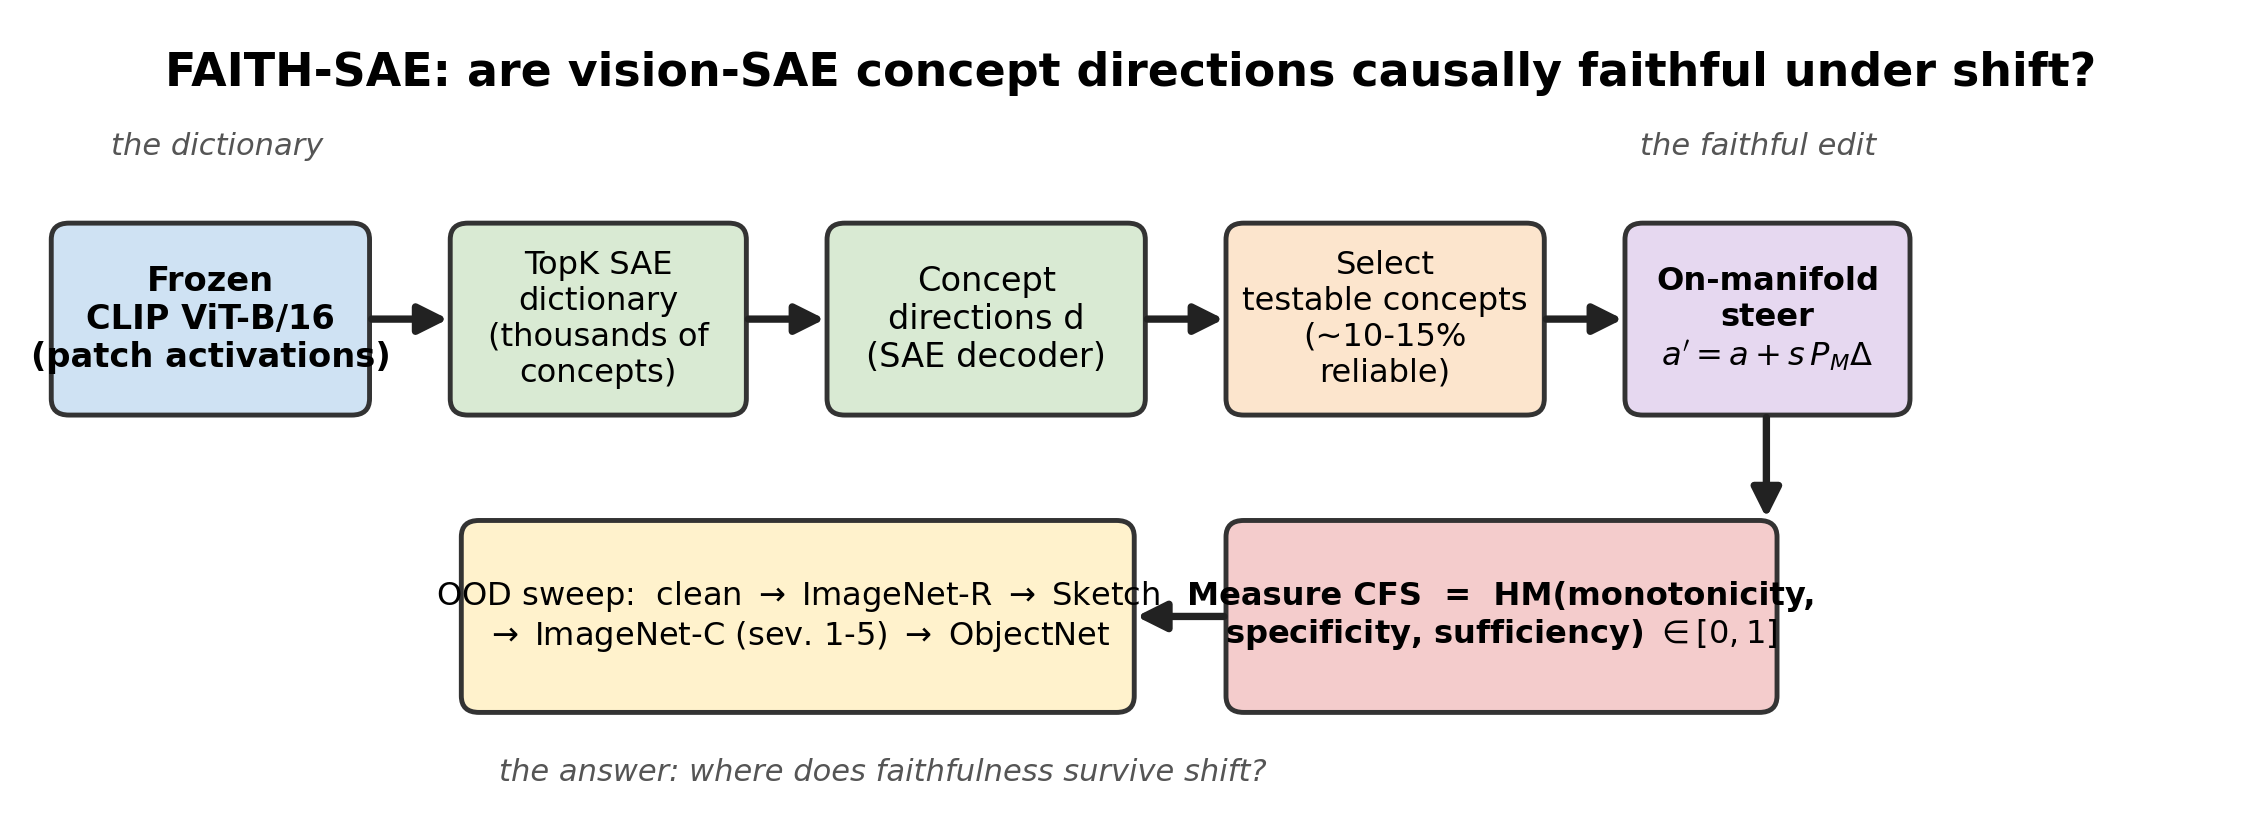
\includegraphics[width=0.97\textwidth]{paper/figures/fig_overview.png}
\caption{\textbf{The big picture.} A \emph{frozen} CLIP ViT-B/16 turns images into activations; a TopK \emph{sparse autoencoder} on its patch activations exposes thousands of \emph{concept directions}. We keep only the well-defined ones (the reliable $\sim$10--15\% tail), \onm{steer them on-manifold} ($P_M\!\cdot\!\Delta$), grade each edit with the \emph{Causal Faithfulness Score} (monotonicity $\times$ specificity $\times$ sufficiency), and then \emph{sweep that score down the out-of-distribution ladder} (clean $\to$ R $\to$ Sketch $\to$ C $\to$ ObjectNet) to see where it survives. \textit{(Numbers in this primer are illustrative teaching examples.)}}
\label{fig:overview}
\end{figure}

% ============================ SECTION 7 ====================================
\section{The idea, step by step}

Now let's walk through what the method actually \emph{does}, slowly. Figure~\ref{fig:method} is the picture to keep in your head.

\begin{enumerate}[leftmargin=1.5em, itemsep=4pt]
  \item \textbf{Pick a concept switch.} From the SAE's thousands of switches, select one that passes an interpretability filter (looks like a clean, single concept). Read off its direction $d$.
  \item \textbf{Build the manifold projector.} From a big pile of real-image activations, compute the top \onm{$r$} directions they vary along; stack them into \onm{$P_M$}. This is the ``allowed surface.''
  \item \textbf{Project the edit.} Form the raw edit $\Delta = s\cdot d$, then trim it to the surface: $\onm{P_M}\cdot\Delta$. Measure how much you trimmed --- the \emph{off-manifold residual} --- as a sanity diagnostic.
  \item \textbf{Apply and read out.} Set the steered activation $a' = a + \onm{P_M}\cdot\Delta$, run the rest of the frozen model, and record two things: the \emph{target} concept's readout, and a panel of \emph{off-target} probes (to catch leakage).
  \item \textbf{Sweep the knob, compute the three components.} Repeat for many strengths $s$. From the resulting curves, compute \emph{monotonicity} (is the rise smooth?), \emph{specificity} (did off-target stay flat?), \emph{sufficiency} (was the effect big?), and combine them into one \textbf{CFS}.
  \item \textbf{Sweep the distribution.} Repeat the whole CFS measurement on each rung of the OOD ladder. Plot CFS versus shift level and mark the collapse knee. That plot is the result.
\end{enumerate}

\begin{figure}[t]
\centering
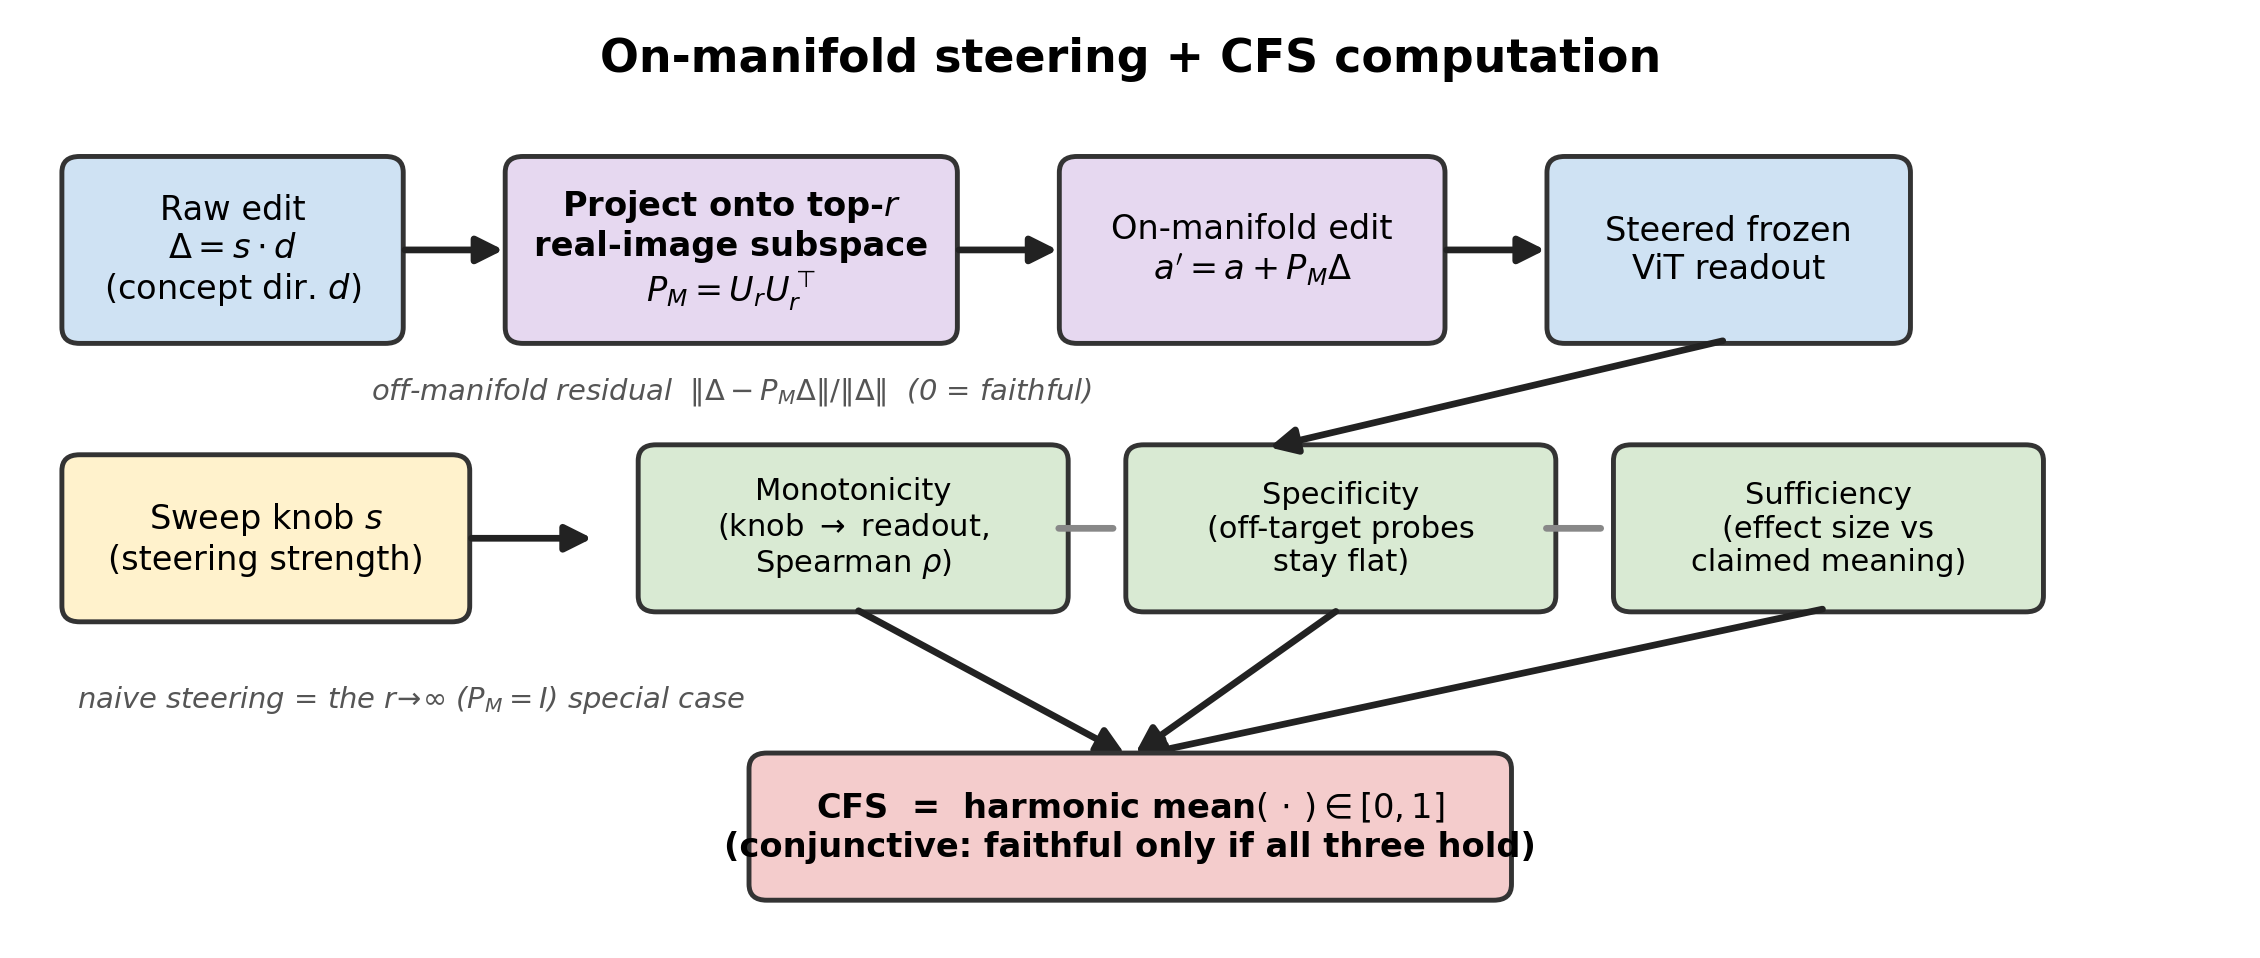
\includegraphics[width=0.95\textwidth]{paper/figures/fig_method.png}
\caption{\textbf{The block, step by step.} A raw edit $\Delta$ is \onm{projected onto the top-$r$ real-image subspace} ($P_M\!\cdot\!\Delta$), scaled by the knob $s$, and added to the frozen activation. The model's \emph{target readout} and \emph{off-target probes} feed the three faithfulness components --- monotonicity, specificity, sufficiency --- which combine (harmonic mean) into a single \emph{Causal Faithfulness Score}. Naive steering is the special case where no projection happens ($P_M = I$).}
\label{fig:method}
\end{figure}

\subsection*{A worked example: the honest run versus the mirage}

Take the same horse photo and the same ``stripes/zebra'' switch from Section 4, but now steer \emph{on-manifold} and compare:

\begin{center}
\renewcommand{\arraystretch}{1.2}
\begin{tabular}{lccccc|c}
\hline
Strength $s$ & 0 & 2 & 4 & 6 & 8 & \textbf{CFS} \\
\hline
\onm{on-manifold} ``zebra'' readout & 0.10 & 0.32 & 0.55 & 0.74 & 0.88 & \onm{\textbf{0.83}} \\
\offm{naive} ``zebra'' readout       & 0.10 & 0.55 & 0.20 & 0.90 & 0.05 & \offm{\textbf{0.12}} \\
\hline
\end{tabular}
\end{center}

The \onm{on-manifold} readout climbs \emph{smoothly and in order} ($0.10\to0.32\to0.55\to0.74\to0.88$): monotonicity is high. If, in addition, the ``ocean'' and ``indoors'' off-target probes barely moved (specificity high) and the final 0.88 is a big jump from 0.10 (sufficiency high), all three components are strong, so their harmonic mean --- the CFS --- is high (\onm{$\approx 0.83$}). The \offm{naive} run bounces, so even though it once hit 0.90, its monotonicity is near zero and the harmonic mean collapses the CFS to \offm{$\approx 0.12$}. \emph{Same switch, same strengths --- the careful edit is faithful; the naive edit is a mirage, and the score says so.}

% ============================ SECTION 8 ====================================
\section{Why it works --- and when it breaks}

\subsection*{Why it works (the intuition)}
Two things line up. First, on-manifold steering removes the single biggest source of \emph{fake} effects --- driving the activation into never-seen territory where the model extrapolates garbage. By keeping the edit on the real-image surface, every readout change is a change a real image could have caused, so it \emph{means} something. Second, the CFS refuses to be fooled by a lucky spike: because it demands monotonicity \emph{and} specificity \emph{and} sufficiency together (via a harmonic mean, which any single near-zero drags down), a jagged or leaky or tiny effect cannot score well. Honest method, suspicious judge: together they yield a trustworthy reading.

\subsection*{When it breaks (be honest)}
On-manifold steering is not magic, and faithfulness is not guaranteed. Here are the honest failure modes:

\begin{itemize}[leftmargin=1.4em, itemsep=3pt]
  \item \textbf{Off-manifold artifact (mostly for the baselines).} Naive and raw-clamp steering routinely leave the manifold; their high apparent effects are non-realistic and undecodable. This is the failure on-manifold steering is built to avoid --- but a too-large rank $r$ can let it creep back.
  \item \textbf{Specificity leakage.} Real SAE directions are rarely perfectly clean. Turning up the target can drag an entangled off-target concept along, especially at high strength. The metric catches it (specificity drops), but it limits how hard you can push.
  \item \textbf{Polysemantic / uninterpretable feature.} Most raw SAE switches ($\sim$85\%) encode several concepts or none clean --- there's simply no honest knob to find. These are filtered out \emph{before} steering, which is why only the $\sim$10--15\% reliable tail is studied.
  \item \textbf{OOD collapse (the headline failure).} A switch faithful on clean photos can lose its meaning on sketches, heavy corruption, or odd real-world scenes --- CFS falls off a cliff past the collapse knee. \emph{Whether and where this happens is the whole point of the measurement.}
  \item \textbf{Magnitude saturation.} Push the knob too far and the readout flattens or clips; monotonicity breaks. There's a knee in the strength sweep beyond which more steering buys nothing real.
\end{itemize}

The unifying lesson: faithfulness is a \emph{measured property, not an assumption}. The two design dials --- steering strength $s$ and projection rank $r$ --- each have a sweet spot, and the OOD ladder tells you how far that sweet spot travels before it falls apart.

% ============================ SECTION 9 ====================================
\section{The simplest math}

Two short formulas carry the whole idea. Here they are, then every symbol explained.

\subsection*{The honesty score}
\begin{equation*}
\boxed{\;\text{CFS} \;=\; \operatorname{HM}\big(\,\text{monotonicity},\;\text{specificity},\;\text{sufficiency}\,\big)\;\in[0,1]\;}
\end{equation*}

\textbf{Term by term:}
\begin{itemize}[leftmargin=1.4em, itemsep=3pt]
  \item \textbf{monotonicity} $\in[0,1]$ --- how smoothly/orderly the readout rises with the knob (rank correlation). \emph{1 = perfectly smooth climb; 0 = bouncing.}
  \item \textbf{specificity} $\in[0,1]$ --- $1$ minus how much \emph{off-target} concepts drifted. \emph{1 = only the target moved; 0 = everything moved.}
  \item \textbf{sufficiency} $\in[0,1]$ --- standardized effect size, ``was it big enough.'' \emph{1 = a decisive effect; 0 = a trivial wiggle.}
  \item \textbf{HM} --- the \emph{harmonic mean}. This is the load-bearing choice: the harmonic mean is small whenever \emph{any one} input is small. So faithfulness is \emph{conjunctive} --- you need smooth \emph{and} specific \emph{and} sufficient, all at once. One failure tanks the score.
\end{itemize}

\textbf{Numbers plugged in.} For three strong components $(0.9, 0.8, 0.85)$:
\[
\text{CFS}=\frac{3}{\frac{1}{0.9}+\frac{1}{0.8}+\frac{1}{0.85}}\approx 0.85 \quad(\text{faithful}).
\]
But if specificity collapses to $0.05$ (the edit leaks everywhere), $(0.9,\,0.05,\,0.85)$ gives
\[
\text{CFS}=\frac{3}{\frac{1}{0.9}+\frac{1}{0.05}+\frac{1}{0.85}}\approx 0.13 \quad(\text{not faithful}).
\]
One bad axis, and the harmonic mean drags the whole score to the floor --- exactly the behaviour we want from an honesty score.

\subsection*{The on-manifold edit}
\begin{equation*}
\boxed{\;a' \;=\; a \;+\; s\cdot(\onm{P_M}\,\Delta),\qquad \onm{P_M} = U_r U_r^{\!\top}\;}
\end{equation*}
\begin{itemize}[leftmargin=1.4em, itemsep=3pt]
  \item $a$ --- the original activation (the model's notes on a real image).
  \item $\Delta = d$ --- the concept's edit direction (the switch's arrow).
  \item $s$ --- the steering strength (how hard we flip the switch).
  \item $U_r$ --- the top-$r$ real-image directions, stacked; \onm{$P_M = U_r U_r^{\top}$} \emph{projects} an arrow onto that real-image surface, trimming the off-manifold part.
  \item $a'$ --- the steered activation, guaranteed to stay near the manifold.
\end{itemize}
\textbf{The unifying punchline:} naive steering is just the special case \onm{$r\to\infty$}, i.e.\ $P_M = I$ (project onto \emph{everything} = trim nothing). On-manifold steering is the same edit with a leash. \emph{(All figures here are illustrative teaching values; real numbers await the CLIP + ImageNet-shift runs.)}

% ============================ SECTION 10 ===================================
\section{How to explain it to others}

This is the payoff. Five ready-made versions for five audiences.

\subsection*{The one-sentence version}
``A tool finds thousands of human-readable concept switches inside a frozen image model, but flipping one naively can fake an effect by pushing the model into nonsense-land; we flip them \emph{carefully} (staying in the space of real images) and score the honesty with one number --- then check whether that honesty survives on weird, out-of-distribution images.''

\subsection*{The one-minute whiteboard version}
\emph{Draw:} a curved line (the manifold = ``places real images live''). Put a dot $a$ on it. Draw a straight arrow shooting \emph{off} the curve --- label it ``\offm{naive: off-manifold, fake effect}.'' Now draw a second arrow that bends to \emph{stay on} the curve --- ``\onm{on-manifold: real effect}.''
\emph{Say:} ``Steering = adding a concept's arrow to the model's notes. Naive steering flies off the curve into settings no photo makes, so the readout is a glitch. We project the arrow back onto the curve, so the edit lands on a \emph{real} spot. Then we grade honesty with three checks --- smooth, on-target, big enough --- multiplied together so one failure tanks the score. Finally we redo it on sketches, blur, and odd scenes, and plot honesty-versus-weirdness: the curve, and where it falls off a cliff, is the answer.''

\subsection*{An analogy for a non-technical friend}
``A car has a dashboard of warning lights, but they're unlabelled. Someone hands you a manual claiming light \#12 means `low oil.' You test it: if you really drain the oil, does light \#12 come on \emph{smoothly}, \emph{by itself}, and \emph{clearly}? Great --- it's honest. But careless testers fake it by ripping out wires (that's `off-manifold' --- no real car ever does that), making lights flicker meaninglessly. We test the lights \emph{the way a real car would behave}, give each light an honesty grade, and then ask: does that honesty still hold in rain, snow, and at night? Because a warning light you can only trust on a sunny test track isn't much use.''

\subsection*{The version for a skeptical expert}
\emph{Precise claim:} Constraining an SAE concept's activation-addition edit to the top-$r$ principal subspace of real-image activations ($a' = a + s\,P_M\Delta$) yields a strictly higher Causal Faithfulness Score --- a harmonic mean of monotonicity, specificity, and sufficiency --- than naive off-manifold ActAdd, raw-clamp, and random-direction steering at \emph{matched steering strength}, on clean ImageNet; and CFS degrades \emph{more gracefully} for on-manifold steering across the shift ladder (R $\to$ Sketch $\to$ C-1..5 $\to$ ObjectNet). The novelty: no prior quantitative faithfulness benchmark for vision-SAE features exists, and none has measured faithfulness under distribution shift.

\emph{The one experiment that convinces them:} a 2-D grid over steering strength $s$ and projection rank $r$, reporting CFS (with bootstrap CIs over concepts) for all five steering methods, then the same swept down ImageNet-C severity 1--5. The decisive sub-plot is \textbf{CFS-vs-shift}: if on-manifold steering sits above naive at matched strength on clean data \emph{and} has a shallower degradation slope with a later collapse knee, the claim holds. A null result (faithfulness collapses for everyone past Sketch) is itself a publishable warning.

\subsection*{Three likely questions, with crisp answers}
\begin{description}[leftmargin=0pt, itemsep=4pt]
  \item[Q: How is a faked effect even possible --- the readout really moved?] Yes, but the model produced that readout while sitting in an activation \emph{no real image creates}, where it's extrapolating blindly. The number changed; it just doesn't \emph{mean} anything. Jagged, non-monotone responses are the tell.
  \item[Q: Why a harmonic mean and not a simple average?] Because faithfulness must be \emph{conjunctive}: a smooth-but-leaky edit, or a specific-but-tiny one, isn't faithful. An average would let a strong axis hide a failing one; the harmonic mean refuses --- any near-zero axis sinks the whole score.
  \item[Q: Why should faithfulness collapse out of distribution at all?] Because the SAE and the manifold were both built from \emph{clean} training images. On a sketch (no texture) or heavy corruption, the activations land in regions the SAE never cleanly mapped and the real-image subspace no longer fits --- so the concept's meaning, and the projector, both degrade. Measuring \emph{where} is the contribution.
\end{description}

% ============================ SECTION 11 ===================================
\section{Glossary}

\begin{description}[leftmargin=0pt, itemsep=3pt]
  \item[Frozen vision model] A fully-trained image model whose weights we never change; we only observe and poke it (e.g.\ CLIP ViT-B/16).
  \item[Activation] The list of numbers a model produces about an image at some internal stage --- its private ``notes.''
  \item[Polysemanticity] The tangling where each activation number mixes many concepts and each concept smears over many numbers.
  \item[Sparse autoencoder (SAE)] A helper network that rewrites a tangled activation as a long list of mostly-off ``concept switches,'' each ideally one clean concept.
  \item[Concept direction] The arrow $d$ in activation space associated with a given SAE switch; adding it turns that concept up.
  \item[Steering] Deliberately flipping a switch ($a' = a + s\,d$) to test whether it \emph{causes} what it claims.
  \item[Steering strength ($s$)] How hard we push the switch.
  \item[Manifold] The thin region of activation space that real images actually produce. \emph{On-manifold} = realistic; \emph{off-manifold} = no real image ever lands there.
  \item[On-manifold steering] Steering with the edit projected onto the real-image subspace ($a' = a + s\,P_M\Delta$), so it stays realistic.
  \item[Projection rank ($r$)] How many real-image directions the leash $P_M$ keeps; the central dial between ``too tight'' and ``too loose.''
  \item[Off-manifold artifact] A readout change caused by extrapolation into never-seen territory --- a fake causal effect.
  \item[CFS (Causal Faithfulness Score)] A single $[0,1]$ honesty score: the harmonic mean of monotonicity, specificity, and sufficiency.
  \item[Monotonicity / Specificity / Sufficiency] The three honesty checks: smooth ordered rise / only-the-target-moves / effect-is-big-enough.
  \item[Out of distribution (OOD)] Test images unlike the clean training set --- renditions, sketches, corruptions, odd real-world scenes.
  \item[Collapse knee] The shift level where CFS falls below a usable floor --- where faithfulness dies.
\end{description}

% ============================ SECTION 12 ===================================
\section{Key takeaways}

\begin{itemize}[leftmargin=1.4em, itemsep=3pt]
  \item A \textbf{sparse autoencoder} turns a frozen vision model's tangled activations into thousands of human-readable \textbf{concept switches} --- but only a small fraction ($\sim$10--15\%) are truly reliable.
  \item Flipping a switch (\textbf{steering}) tests cause, but a \emph{naive} edit can fly \textbf{off-manifold} into settings no real image makes, producing a \emph{fake} effect that only \emph{looks} real.
  \item \textbf{On-manifold steering} projects the edit onto the real-image subspace ($a' = a + s\,P_M\Delta$), keeping it realistic --- so the effect is genuine.
  \item The \textbf{Causal Faithfulness Score} grades honesty with one number, the harmonic mean of \emph{monotonicity}, \emph{specificity}, and \emph{sufficiency} --- conjunctive, so one failure tanks it.
  \item The two halves complete each other: the careful method gives the metric something \emph{real} to measure; the metric \emph{proves} the method faithful and \emph{tracks where it breaks}.
  \item The headline result is one curve: \textbf{CFS versus distribution shift} (clean $\to$ R $\to$ Sketch $\to$ C $\to$ ObjectNet), with its \textbf{collapse knee} --- telling us whether vision-SAE interpretability can be trusted in the messy real world.
\end{itemize}

\vspace{0.8em}
\hrule
\vspace{0.6em}
\begin{center}
\small\textcolor{graytext}{Numbers in this primer are illustrative teaching examples; this document reports no experimental results. \\ The \emph{idea} it teaches is final.}
\end{center}

\end{document}
